Хотим построить лист $x^{(j)} < t$. Хотим ввести какую-то характерестику <<гетерогенности>> $H$ и мимнимизировать выражение 

\[ \frac{|L|}{|Q|} H(L) + \frac{|R|}{|Q|} H(R) \rightarrow min_{j, t},\]

где $Q$ - множество, которое разбивается этим листом, а $L, R$ - части, на которое оно разбивается

Более простым языком: $H$ - показывает насколько сильный разброс данных в этом множестве (чем он меньше, тем ближе все данные будут к предсказанному значению).

\begin{definition}
    Функция $H$ называется \textit{критерием информативности} (information criteria)
\end{definition}

Есть разные способы задать $H$ для задачи классификации. Посмотрим сначала на примере бинарной классификации. Далее $p_i$ - нормированная частота встречаемости $i$-ого класса в множестве $R$

\begin{enumerate}
    \item Misclassification criteria: количество ошибок классфикации (предсказываем доминирующий класс и смотрим сколько объектов классифицировали неправильно)

    \[ H(R) = 1 - \max\{p_0, p_1\}\]

    Не очень хороший способ: например для многоклассовой классификации дерево может хорошо отделять несколько каких-то классов от остальных, но этот критерий нам этого не покажет

    \item Entropy criteria

    \[ H(R)=-p_0 \log p_0 - p_1 \log p_1 = -p_0 \log p_0 - (1-p_0) \log (1-p_0)\]

    Энтропия <<на пальцах>>: чем больше энтропия, тем больше хаоса

    \item Gini impurity

    \[ H(R)=1 - p_0^2 - p_1^2 = 1 - p_0^2 - (1-p_0)^2=2p_0 (1- p_0)\]

    Интуитивно: берем два объекта из нашей подвыборки. Какова вероятность, что они окажутся разных классов?
\end{enumerate}

Для многоклассовой классификации аналогично

\begin{enumerate}
    \item Misclassification: $H(R)=1- \max \{ p_0, \ldots, p_k \}$

    \item Entropy: $H(R)=-\sum_{i=0}^k p_i \log p_i$

    \item Gini: $H(R)=1 - \sum_{i=0}^k p_i^2$
\end{enumerate}

\begin{figure}[H]

\centering

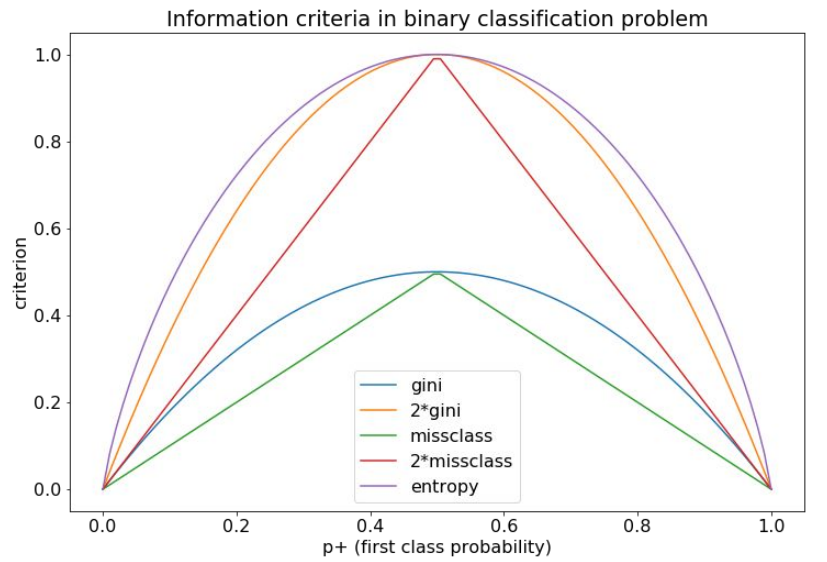
\includegraphics[width=0.6\linewidth]{images/information criteria.png}

\caption{График разных критериев информативности}

\end{figure}

Из графика выше видим, что энтропия и Джини ведут себя примерно одинаково и на практике не очень отличаются (вроде в последнее время чаще используют Джини). Так же график показывает, что misclassification слишком мало штрафует за малые ошибки (по сравнению с остальными критериями)

Для задачи регрессии нам придется взять другой критерий информативности (mean squared error)

\[ H(R) = \min_c \frac 1 {|R|} \sum_{(x_i, y_i) \in R} (y_i - c)^2\]

Оптимальная константа (оценка максимального правдоподобия на $c$): 

\[ c^*=\frac 1 {|R|} \sum_{y_i \in R} y_i \]

Интуитивно: считаем дисперсию относительно среднего

Вопрос <<со звёздочкой>>: если оптимизируем MAE, то $c^*$ --- это медиана

Подробнее про то, почему получаются такие оценки можно почитать \href{https://d18ky98rnyall9.cloudfront.net/rpPnDwIOSFaT5w8CDnhWWA_44e3f19ed9fd4e56baa1c8ce9ba064b5_loss_functions.pdf?Expires=1673308800&Signature=Bpev8rp2H1yc4cLEgoHJVJyO~3J-4z0SR9hTDea8xAZfKECVNgdr7bG~N33xj71vSyGs8jOkXWwZKRw-q2x5wTxxQDPsiV7K71MAItbktK83ranmPjApYcBipi9rimYRQAoLwKOBZr5RtF0DEiF7FXr5HaBuh4KXCQMnOYSqoFs_&Key-Pair-Id=APKAJLTNE6QMUY6HBC5A}{здесь} 